\let\lesson\undefined
\newcommand{\lesson}{\phantomlesson{Bài 5.}}
\setcounter{section}{2}
\section{Bài tập trắc nghiệm}
\begin{enumerate}[label=\bfseries Câu \arabic*:,leftmargin=1.5cm]
	\item \mkstar{2}\\
	{Một hành khách ngồi trong xe A, nhìn qua cửa sổ thấy xe B bên cạnh và sân ga đều chuyển động như nhau. Như vậy
	\begin{mcq}(2)
		\item xe A đứng yên, xe B chuyển động.
		\item xe A chạy, xe B đứng yên.
		\item xe A và xe B chạy cùng chiều.
		\item xe A và xe B chạy ngược chiều.
	\end{mcq}
}
\hideall{
\textbf{Đáp án: B.}
}

\item \mkstar{2}\\
{Chọn phát biểu \textbf{sai}:
\begin{mcq}
	\item Vận tốc của chất điểm phụ thuộc vào hệ qui chiếu.
	\item Trong các hệ qui chiếu khác nhau thì vị trí của cùng một vật là khác nhau.
	\item Khoảng cách giữa hai điểm trong không gian là tương đối.
	\item Tọa độ của một chất điểm phụ thuộc hệ qui chiếu.
\end{mcq}
}
\hideall{
\textbf{Đáp án: C.}\\
Khoảng cách giữa hai điểm trong không gian không phụ thuộc vào hệ quy chiếu.
}

\item \mkstar{2}\\
{Chọn câu đúng, đứng ở Trái Đất ta sẽ thấy:
\begin{mcq}
	\item Trái Đất đứng yên, Mặt Trời và Mặt Trăng quay quanh Trái Đất.
	\item Mặt Trời đứng yên, Trái Đất quay quanh Mặt Trời, Mặt trăng quay quanh Trái đất.
	\item Mặt Trời đứng yên, Trái Đất và Mặt Trăng quay quanh Mặt Trời.
	\item Mặt Trời và mặt đất đứng yên, Mặt Trăng quay quanh Trái Đất.
\end{mcq}
}
\hideall{
\textbf{Đáp án: A.}
}

\item \mkstar{2}\\
{Một hành khách ngồi trong toa tàu H, nhìn qua cửa sổ thấy toa tàu N bên cạnh và gạch lát sân ga đều chuyển động như nhau. Hỏi toa tàu nào chạy?
\begin{mcq}(2)
	\item Tàu N chạy tàu H đứng yên.
	\item Cả 2 tàu đều chạy.
	\item Tàu H chạy tàu N đứng yên.
	\item Cả 2 tàu đều đứng yên.
\end{mcq}
}
\hideall{
\textbf{Đáp án: C.}
}

\item \mkstar{2}\\
{Biết vận tốc của ca nô so với mặt nước đứng yên là $\SI{10}{\meter/\second}$. Vận tốc của dòng nước là $\SI{4}{\meter/\second}$. Tính vận tốc của ca nô khi
\begin{enumerate}[label=\alph*)]
	\item ca nô đi xuôi dòng.
	\begin{mcq}(4)
		\item $\SI{14}{\meter/\second}$.
		\item $\SI{9}{\meter/\second}$.
		\item $\SI{6}{\meter/\second}$.
		\item $\SI{5}{\meter/\second}$.
	\end{mcq}
\item ca nô đi ngược dòng.
\begin{mcq}(4)
	\item $\SI{14}{\meter/\second}$.
	\item $\SI{9}{\meter/\second}$.
	\item $\SI{6}{\meter/\second}$.
	\item $\SI{5}{\meter/\second}$.
\end{mcq}
\end{enumerate}

}
\hideall{
\textbf{Đáp án: A - C.}
}

\item  \mkstar{3}\\
{Hai ô tô A và B chạy cùng chiều trên cùng một đoạn đường với vận tốc $\SI{70}{\kilo\meter/\hour}$ và $\SI{65}{\kilo\meter/\hour}$. Vận tốc của ô tô A so với ô tô B bằng
	\begin{mcq}(4)
		\item $\SI{30}{\kilo\meter/\hour}$.
		\item $\SI{5}{\kilo\meter/\hour}$.
		\item $\SI{135}{\kilo\meter/\hour}$.
		\item $\SI{65}{\kilo\meter/\hour}$.
	\end{mcq}

}
\hideall{
\textbf{Đáp án: B.}
}

\item \mkstar{3}\\
{A ngồi trên một toa tàu chuyển động với vận tốc $\SI{15}{\kilo\meter/\hour}$ đang rời ga. B ngồi trên một toa tàu khác chuyển động với vận tốc $\SI{10}{\kilo\meter/\hour}$ đang đi ngược chiều vào ga. Hai đường tàu song song với nhau. Chọn chiều dương là chiều chuyển động của đoàn tàu mà A ngồi. Tính vận tốc của B đối với A.
	\begin{mcq}(4)
		\item $\SI{-5}{\kilo\meter/\hour}$.
		\item $\SI{5}{\kilo\meter/\hour}$.
		\item $\SI{25}{\kilo\meter/\hour}$.
		\item $\SI{-25}{\kilo\meter/\hour}$.
	\end{mcq}

}
\hideall{
\textbf{Đáp án: D.}\\
Chọn chiều dương là chiều chuyển động của tàu A.

$\overrightarrow{v_\text{AD}}$ là vận tốc của tàu A đối với đất;

$\overrightarrow{v_\text{BD}}$ là vận tốc của tàu B đối với đất;

$\overrightarrow{v_\text{BA}}$ là vận tốc của tàu B đối với tàu A.

Theo công thức cộng vận tốc:
$$\overrightarrow{v_\text{BD}} = \overrightarrow{v_\text{BA}}+\overrightarrow{v_\text{AD}} \Rightarrow \overrightarrow{v_\text{BA}} = \overrightarrow{v_\text{BD}} - \overrightarrow{v_\text{AD}}=\overrightarrow{v_\text{BD}} + \overrightarrow{-v_\text{AD}}$$

Chiếu lên chiều chuyển động của tàu A:
$$v_\text{AB} = -v_\text{BD} - v_\text{AD} = -10-15 = \SI{-25}{km/h}$$

Vận tốc của tàu B đối với tàu A có độ lớn $\SI{25}{km/h}$ và ngược chiều so với chiều chuyển động của tàu A.
}

\item \mkstar{3}\\
{Hai bến sông A và B cùng nằm trên một bờ sông, cách nhau $\SI{18}{\kilo\meter}$. Cho biết độ lớn vận tốc của ca nô đối với nước là $u =\SI{16.2}{\kilo\meter/\hour}$ và độ lớn vận tốc của nước đối với bờ sông là $v=\SI{5.4}{\kilo\meter/\hour}$. Thời gian để ca nô chạy xuôi dòng từ A đến B rồi lại chạy ngược dòng trở về A là
\begin{mcq}(4)
	\item 1 giờ 40 phút.
	\item 1 giờ 20 phút.
	\item 2 giờ 30 phút.
	\item 2 giờ 10 phút.
\end{mcq}
}
\hideall{
\textbf{Đáp án: C.}\\
Thời gian ca nô chạy xuôi dòng từ A đến B rồi chạy ngược lại trở về A:
$$t=\dfrac{s}{u+v}+\dfrac{s}{u-v}=\SI{2.5}{\second}.$$
}

\item \mkstar{3}\\
{Ô tô A chạy thẳng về hướng Tây với độ lớn vận tốc $\SI{40}{\kilo\meter/\hour}$. Ô tô B chạy thẳng về hướng Bắc với độ lớn vận tốc $\SI{60}{\kilo\meter/\hour}$. Độ lớn vận tốc của ô tô B so với người ngồi trên ô tô A gần giá trị nào nhất sau đây?
\begin{mcq}(4)
	\item $\SI{85}{\kilo\meter/\hour}$.
	\item $\SI{90}{\kilo\meter/\hour}$.
	\item $\SI{65}{\kilo\meter/\hour}$.
	\item $\SI{75}{\kilo\meter/\hour}$.
\end{mcq}
}
\hideall{
\textbf{Đáp án: D.}\\
Vận tốc của ô tô B đới với người ngồi trên ô tô A:
$$\overrightarrow{v_{BA}}=\overrightarrow{v_{BD}}-\overrightarrow{v_{AD}}$$
Vì $\overrightarrow{v_{BD}}\bot \overrightarrow{v_{AD}}$ nên
$$v_{BA}=\sqrt{v^2_{BD}+v^2_{AD}}\approx\SI{72}{\kilo\meter/\hour}$$
}

\item \mkstar{4}\\
{Một người lái xuồng máy cho xuồng chạy ngang con sông rộng $\SI{240}{\meter}$. Mũi xuồng luôn luôn vuông góc với bờ sông, nhưng do nước chảy nên xuồng sang đến bờ bên kia tại một điểm cách bến dự định $\SI{180}{\meter}$ về phía hạ lưu và xuồng đi hết 1 phút. Độ lớn vận tốc của xuồng so với bờ là
\begin{mcq}(4)
	\item $\SI{8}{\meter/\second}$.
	\item $\SI{9}{\meter/\second}$.
	\item $\SI{6}{\meter/\second}$.
	\item $\SI{5}{\meter/\second}$.
\end{mcq}
}
\hideall{
\textbf{Đáp án: D.}\\
Độ dịch chuyển của xuồng so với vị trí ban đầu:
$$d=\sqrt{240^2+180^2}=\SI{300}{\meter}$$
Độ lớn vận tốc của xuồng so với bờ:
$$v_{xd}=\dfrac{d}{t}=\SI{5}{\meter/\second}.$$
}
\end{enumerate}
\section{Bài tập tự luận}
\begin{enumerate}[label=\bfseries Bài \arabic*:,leftmargin=1.5cm]
	\item \mkstar{3}\\
	{Biết $\overrightarrow{d_1}$ là độ dịch chuyển $\SI{10}{\meter}$ về phía đông còn $\overrightarrow{d_2}$ là độ dịch chuyển $\SI{6}{\meter}$ về phía tây. Hãy xác định độ dịch chuyển tổng hợp trong 2 trường hợp sau
		\begin{enumerate}[label=\alph*)]
			\item $\overrightarrow{d}=\overrightarrow{d_1}+\overrightarrow{d_2}$.
			\item $\overrightarrow{d}=\overrightarrow{d_1}+3\overrightarrow{d_2}$.
		\end{enumerate}
		
	}
	\hideall{
		\begin{enumerate}[label=\alph*)]
			\item $d=\SI{4}{\meter}$ về hướng đông.
			\item $d=\SI{8}{\meter}$ về hướng tây
		\end{enumerate}
	}

	\item \mkstar{3}
	
	{Một ô tô A chạy đều trên một đường thẳng với vận tốc $\SI{40}{km/h}$. Một ô tô B đuổi theo ô tô A với vận tốc $\SI{60}{km/h}$. Xác định vận tốc của ô tô B đối với ô tô A và của ô tô A đối với ô tô B.}
	\hideall{
		Chọn chiều dương là chiều chuyển động của hai xe.
		
		$\overrightarrow{v_\text{AD}}$ là vận tốc của xe A đối với đất;
		
		$\overrightarrow{v_\text{BD}}$ là vận tốc của xe B đối với đất;
		
		$\overrightarrow{v_\text{BA}}$ là vận tốc của xe B đối với xe A.
		
		Theo công thức cộng vận tốc:
		$$\overrightarrow{v_\text{AB}} = \overrightarrow{v_\text{AD}}+\overrightarrow{v_\text{DB}} \Rightarrow \overrightarrow{v_\text{AB}} = \overrightarrow{v_\text{AD}} - \overrightarrow{v_\text{BD}}$$
		
		Chiếu lên hướng chuyển đông của ô tô A:
		$$v_\text{AB} = 40-60=-20\ \text{km/h}$$
		
		Vậy $v_\text{BA} = 20\ \text{km/h}$.
	}
	
	\item \mkstar{3}
	
	
	{   
		Trên đoàn tàu đang chạy thẳng với vận tốc trung bình $\SI{36}{km/h}$ so với mặt đường. Hãy xác định vận tốc của hành khách đối với mặt đường nếu người này chuyển động về cuối đoàn tàu với vận tốc có cùng độ lớn $\SI{1}{m/s}$.
	}
	\hideall
	{
		
		Đổi: $\SI{36}{km/h} = \SI{10}{m/s}$.
		
		Gọi:
		
		$\vec v_{1,2}$ là vận tốc của hành khách so với tàu.
		
		$\vec v_{2,3}$ là vận tốc của tàu so với mặt đường.
		
		$\vec v_{1,3}$ là vận tốc của hành khách so với mặt đường.
		
		Ta có:
		
		$$\vec v_{1,3} = \vec v_{1,2} + \vec v_{2,3}.$$
		
		Chọn chiều chuyển động của tàu đối với đất làm chiều dương:
		
		$$v_{1,3} = - v_{1,2} + v_{2,3} = \SI{9}{m/s}.$$
		
		
	}

	\item \mkstar{3}
	
	
	{
		Trên đoàn tàu đang chạy thẳng với vận tốc trung bình $\SI{36}{km/h}$ so với mặt đường, một hành khách đi về đầu tàu với vận tốc $\SI{1}{m/s}$ so với mặt sàn tàu.
		\begin{center}
			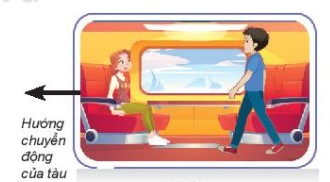
\includegraphics[scale=1]{../figs/VN10-2022-PH-TP005-3.jpg}
		\end{center}
		\begin{enumerate}[label=\alph*)]
			\item Hành khách này tham gia mấy chuyển động?
			\item Làm cách nào để xác định được vận tốc của hành khách đối với mặt đường?
		\end{enumerate}
	}
	\hideall
	{
		\begin{enumerate}[label=\alph*)]
			\item Hành khách này tham gia 2 chuyển động: Chuyển động với vận tốc $\SI{1}{m/s}$ so với sàn tàu và chuyển động do tàu kéo đi với vận tốc bằng vận tốc của tàu so với mặt đường. Chuyển động của hành khách so với mặt đường là tổng hợp của hai chuyển động trên.
			\item Gọi:
			
			- $\vec v_{1,2}$ là vận tốc của hành khách so với tàu.
			
			- $\vec v_{2,3}$ là vận tốc của tàu so với mặt đường.
			
			- $\vec v_{1,3}$ là vận tốc của hành khách so với mặt đường.
			
			Thì:
			
			$$\vec v_{1,3} = \vec v_{1,2} + \vec v_{2,3}$$
			
			Chọn chiều chuyển động của tàu làm chiều dương:
			
			$$v_{1,3} = v_{1,2} + v_{2,3} = \SI{11}{m/s}.$$
			
			Hướng của vận tốc người so với mặt đường là hướng đoàn tàu chạy.
		\end{enumerate}
	}

	\item \mkstar{3}
	
	
	{
		Một người bơi trong bể bơi yên lặng có thể đạt tới vận tốc $\SI{1}{m/s}$. Nếu người này bơi xuôi dòng sông có dòng chảy với vận tốc $\SI{1}{m/s}$ thì có thể đạt vận tốc tối đa là bao nhiêu?
	}
	\hideall
	{
		Gọi:
		
		$\vec v_{1,2}$ là vận tốc của người so với nước.
		
		$\vec v_{2,3}$ là vận tốc của nước so với bờ.
		
		$\vec v_{1,3}$ là vận tốc của người so với bờ.
		
		Ta có:
		
		$$\vec v_{1,3} = \vec v_{1,2} + \vec v_{2,3}.$$
		
		- Khi người bơi trong bể nước yên lặng, thì $v_{2,3} = 0$:
		
		$$v_{1,2} = v_{1,3} = \SI{1}{m/s}.$$
		
		- Khi người này bơi xuôi dòng chảy với vận tốc $v_{2,3} = \SI{1}{m/s}$:
		
		
		$$v_{1,3} = v_{1,2} + v_{2,3} = \SI{2}{m/s}.$$
		
		Vậy nếu người này bơi xuôi dòng sông có dòng chảy với vận tốc $\SI{1}{m/s}$ thì có thể đạt vận tốc tối đa là $\SI{2}{m/s}.$
		
		
	}
	\item \mkstar{3}
	
	
	{
		Một ca nô chạy hết tốc lực trên mặt nước yên lặng có thể đạt $\SI{21,5}{km/h}$. Ca nô này chạy xuôi dòng sông trong 1 giờ rồi quay lại thì phải mất 2 giờ nữa mới về tới vị trí ban đầu. Hãy tính vận tốc chảy của dòng sông.
	}
	\hideall
	{
		Gọi:
		
		$\vec v_{1,2}$ là vận tốc của canô so với nước.
		
		
		$\vec v_{2,3}$ là vận tốc của nước so với bờ.
		
		
		$\vec v_{1,3}$ là vận tốc của canô so với bờ.
		
		Ta có:
		
		$$\vec v_{1,3} = \vec v_{1,2} + \vec v_{2,3}.$$
		
		- Khi canô chạy trên mặt nước yên lặng, tức $v_{2,3} = 0$:
		
		
		$$v_{1,2} = v_{1,3} = \SI{21,5}{km/h}.$$
		
		- Khi canô chạy xuôi dòng sông, ta có:
		
		$$v_{1,3} = v_{1,2} + v_{2,3} =\dfrac{d}{t_1}$$
		
		- Khi canô quay lại, ta có:
		
		$$v'_{1,3} = v_{1,2} - v_{2,3} =\dfrac{d}{t_2}$$
		
		Thay các đại lượng của đề vào (1) và (2) ta suy ra:
		
		$$\begin{cases}
			d = \SI{28,67}{km}.\\
			v_{2,3} = \SI{7,17}{km/h}.
		\end{cases}$$
		
		Vậy vận tốc chảy của dòng sông là $\SI{7,17}{km/h}$.
		
		
	}
	\item \mkstar{3}
	
	
	{
		Một ca nô chạy trong hồ nước yên lặng có vận tốc tối đa $\SI{18}{km/h}$. Nếu ca nô chạy ngang một con sông có dòng chảy theo hướng Bắc - Nam với vận tốc lên tới $\SI{5}{m/s}$ thì vận tốc tối đa nó có thể đạt được so với bờ sông là bao nhiêu và theo hướng nào?
	}
	\hideall
	{
		\begin{center}
			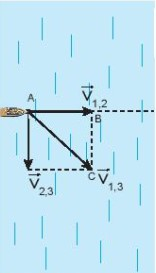
\includegraphics[scale=1]{../figs/VN10-2022-PH-TP005-4.jpg}
		\end{center}
		Gọi vận tốc của ca nô đối với mặt nước là $\vec v_{1,2}$; 
		
		Vận tốc của nước chảy đối với bờ sông là $\vec v_{2,3}$. 
		
		Vận tốc của ca nô đối với bờ sông:
		
		$$\vec v_{1,3} = \vec v_{1,2} + \vec v_{2,3}.$$
		
		Suy ra:
		
		$$v_{1,3} = \sqrt{ v_{1,2}^2 + v_{2,3}^2} = \SI{7,07}{m/s}.$$
		
		Vì $\text{AB} = \text{BC}$ nên tam giác ABC là tam giác vuông cân và góc A bằng $45^\circ$. Hướng của vận tốc nghiêng $45^\circ$ theo hướng Đông - Nam.
	}
	\item \mkstar{3}
	
	
	{
		Một máy bay đang bay theo hướng Bắc với vận tốc $\SI{200}{m/s}$ thì bị gió từ hướng Tây thổi vào với vận tốc $\SI{20}{m/s}$. Xác định vận tốc tổng hợp của máy bay lúc này.
	}
	\hideall
	{
		Gọi:
		
		$\vec v_{1,2}$ là vận tốc của máy bay so với gió.
		
		$\vec v_{2,3}$ là vận tốc của gió so với đường bay.
		
		$\vec v_{1,3}$ là vận tốc của máy bay so với đường bay.
		
		Ta có:
		
		$$\vec v_{1,3} = \vec v_{1,2} + \vec v_{2,3}.$$
		
		Vận tốc tổng hợp của máy bay lúc này là
		
		$$v_{1,3} = \sqrt{v_{1,2}^2 + v^2_{2,3}} = \SI{201}{m/s}.$$
		Vận tốc tổng hợp hướng theo hướng Tây - Bắc hợp với hướng Nam - Bắc 1 góc 
		$$\tan\alpha=\dfrac{v_{23}}{v_{12}}=\dfrac{1}{10}\Rightarrow \alpha =\SI{5.7}{\degree}.$$
	}
		

\item \mkstar{3}\\
{Một người bơi từ bờ này sang bờ kia của một con sông rộng $\SI{50}{\meter}$ theo hướng vuông góc với bờ sông. Do nước sông chảy mạnh nên quãng đường người đó bơi gấp 2 lần so với khi bơi trong bể bơi.
	\begin{enumerate}[label=\alph*)]
		\item Hãy xác định độ dịch chuyển của người này khi bơi sang bờ sông bên kia.
		\item Vị trí điểm tới cách điểm đối diện với điểm khởi hành của người bơi là bao nhiêu mét?
	\end{enumerate}
	
}
\hideall{
	\begin{center}
		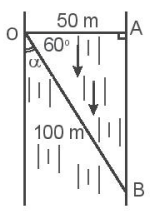
\includegraphics[width=0.15\linewidth]{../figs/VN10-2023-PH-TP0002-6}
	\end{center}
	\begin{enumerate}[label=\alph*)]
		\item $d=\SI{100}{\meter}$ theo hướng làm với bờ sông một góc $\alpha=\SI{30}{\degree}$.
		\item $AB=OA\tan\SI{60}{\degree}=\SI{86.6}{\meter}$.
	\end{enumerate}
}

\item \mkstar{3}\\
{Một người chèo thuyền qua một con sông rộng $\SI{400}{\meter}$. Muốn cho thuyền đi theo đường AB thì người đó phải luôn hướng mũi thuyền theo hướng AC. Biết thuyền qua sông hết $\SI{8}{\minute} \SI{20}{\second}$ và tốc độ của dòng nước là $\SI{0.6}{\meter/\second}$. Tìm tốc độ của thuyền so với dòng nước.
	\begin{center}
		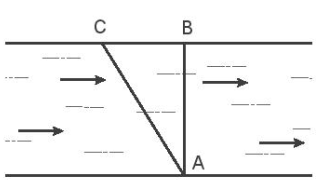
\includegraphics[width=0.35\linewidth]{../figs/VN10-2023-PH-TP0002-7}
	\end{center}
	
}
\hideall{
	Quãng đường nước đẩy thuyền trôi:
	$$BC=v_n\cdot t=\SI{300}{\meter}$$
	Tốc độ của thuyền so với dòng nước:
	$$v_\text{thuyền/nước}=\dfrac{AC}{t}=\dfrac{\sqrt{AB^2+BC^2}}{t}=\SI{1}{\meter/\second}.$$
}

\end{enumerate}
